\documentclass{article}
\usepackage{fancyhdr}
\usepackage{graphicx}
\usepackage{needspace}
\usepackage{amsthm,amssymb,amsmath}
\usepackage{fancyvrb}
\usepackage{tikz}
\usepackage{pgfplots}
\usepackage[section]{placeins}
\usepackage{float}
\usepackage{caption}
\usepackage{enumitem}
\usepackage{hyperref}
\usetikzlibrary{arrows, automata}

\pgfplotsset{compat=newest}
\renewcommand\qedsymbol{$\blacksquare$}
\pagestyle{fancy}

\fancyhf{}
\rhead{FALL 2019}
\lhead{CS440 - ASSIGNMENT 2}
\rfoot{\thepage}

\newtheorem{theorem}{Theorem}

\begin{document}

\begin{titlepage}
    \begin{center}
        \vspace*{1cm}
 
        \Huge
        \textbf{Assignment 2}
 
        \vspace{0.5cm}
        \LARGE
        Search Problems in AI
 
        \vspace{1.5cm}
 
        \vspace{0.8cm}
  
        \Large
        Fall 2019\\
        Rutgers University\\
        CS440: Introduction to Artificial Intelligence\\
       	
       	\vspace{2cm}
        \large
        \textbf{Group Members} \\
        Joshua Rozenberg (jr922)\\
        JohnRobert Delos Santos (jad537)\\
   
    \end{center}
\end{titlepage}

\newpage
\pagenumbering{arabic}

\section{Tracing A* Search}
Using the convention ($city$, $f(city)$, $g(city)$, $h(city)$), we trace the A* search from Lugoj to Bucharest.\\\\
\textbf{Start:} (Lugoj, 244, 0, 244), \textbf{expand Lugoj}.\\
(Mehadia, 311, 70, 241), (Timisoara, 440, 111, 329), \textbf{expand Mehadia}.\\
(Drobeta, 387, 145, 242), \textbf{expand Drobeta}.\\
(Craiova, 425, 265, 160), \textbf{expand Craiova}.\\
(Rimnicu Vilcea, 604, 411, 193), (Pitesti, 503, 403, 100), \textbf{expand Timisoara}.\\
(Arad, 595, 229, 336), \textbf{expand Pitesti}.\\
(Bucharest, 504, 504, 0), \textbf{expand Bucharest}.\\
\textbf{Goal state found.}\\
Sequence of expanded nodes is $Lugoj \rightarrow Mehadia \rightarrow Drobeta \rightarrow Craiova \rightarrow Timisoara \rightarrow Pitesti \rightarrow Bucharest$.
\section{Tracing Other Searches}
Consider a state space where the start state is number 1 and each state \textit{k} has two successors: numbers $2k$ and $2k+1$. Let goal state be 11. From left to right, we have the order of nodes visited for breadth-first search, depth-limited search with limit 3, iterative deepening, and bidirectional search.
\begin{center}
\begin{tikzpicture}[level distance=1.25cm,
  level 1/.style={sibling distance=5cm},
  level 2/.style={sibling distance=2.5cm},
  level 3/.style={sibling distance=1.5cm}]
  \node {1}
    child {node {2}
      child {node {4} child {node {8}} child {node {9}}}
      child {node {5} child {node {10}} child {node {11}}}
    }
    child {node {3}
    child {node {6} child {node {12}} child {node {13}}}
      child {node {7} child {node {14}} child {node {15}}}
    };
\end{tikzpicture}
\end{center}
a)\\ \textbf{BFS:} (1)(2)(3)(4)(5)(6)(7)(8)(9)(10)(11)
\\
\textbf{Depth-limited w/ limit 3:} (1)(2)(4)(8)(9)(5)(10)(11)
\\
\textbf{Iterative deepening:} (1); (1)(2)(3); (1)(2)(4)(5)(3)(6)(7); (1)(2)(4)(8)(9)(5)(10)(11)
\\
b)\\ Bidirectional search would work well on this problem because the successor of n in the reverse direction is n/2. If we were to run bidirectional search on the graph, we'd get:
\\
\textbf{Forward} (1), (2)(3), (4)(5)
\textbf{Backward} (11), (5)
\\
This would give a branching factor of 2 in the forward direction and a branching factor of 1 in the backward direction.

\section{True or False?}
\textit{Which of the following statements are correct and which ones are wrong?}

\begin{enumerate}[label=(\alph*)]
\item Breadth-first search is a special case of uniform-cost search. \textbf{True.}
\item Depth-first search is a special case of best-first tree search. \textbf{False.} 
\item Uniform-cost search is a special case of A* search. \textbf{True.}
\item Depth-first graph search is guaranteed to return an optimal solution. \textbf{False.}
\item Breadth-first graph search is guaranteed to return an optimal solution. \textbf{False.}
\item Uniform-cost graph search is guaranteed to return an optimal solution. \textbf{True.}
\item A* graph search is guaranteed to return an optimal solution if the heuristic is consistent. \textbf{True.}
\item A* graph search is guaranteed to expand no more nodes than depth-first graph search if the heuristic is consistent. \textbf{False.}
\item A* graph search is guaranteed to expand no more nodes than uniform-cost graph search if the heuristic is consistent. \textbf{True.}
\end{enumerate}

\section{Iterative Deepening vs BFS}
\textit{Iterative deepening is sometimes used as an alternative to breadth first search.  Give one advantage of iterative deepening over BFS, and give one disadvantage of iterative deepening as compared with BFS.}
\\\\
One advantage of iterative deepening over BFS is that it will take up less memory. Let b = maximum branching factor and d = depth of shallowest goal state, then space complexity of BFS is $O(b^d)$ compared to that of iterative deepening which is $O(bd)$. A disadvantage is that iterative deepening may expand previously visited states again since it repeats the work done by the previous search. In comparison, BFS will only expand every state once.
\newpage
\section{Heuristics I}
\textit{Prove that if a heuristic is consistent, it must be admissible. Construct an example of an admissible heuristic that is not consistent.}
\begin{proof}
We can prove this through proof of contradiction. Let us assume h(n) is consistent and not admissible. Recall that h'(n) is the true path cost of n.
\begin{align*}
\forall (n,a,n'): h(n) \leq c(n,a,n') + h(n')\\
\neg[\forall n: h(n) \leq h'(n)] \rightarrow \exists n: h(n) > h'(n)
\end{align*}
Let g be the goal state, h(g) = 0, then we can get the following.
\begin{align*}
\forall (n,a,g): h(n) \leq c(n, a, g) + 0 = c(n, a, g) \\
\forall (n,a,g): h(n) \leq c(n, a, g)
\end{align*}
Since c(n, a, g) is the true path cost of g, we have.
\begin{align*}
c(n, a, g) = h'(g) \\
\forall (g): h(g) \leq h'(g)
\end{align*}
This contradicts the property that h(n) is not admissible so h(n) must be admissible if it is consistent.
\end{proof}
\begin{center}
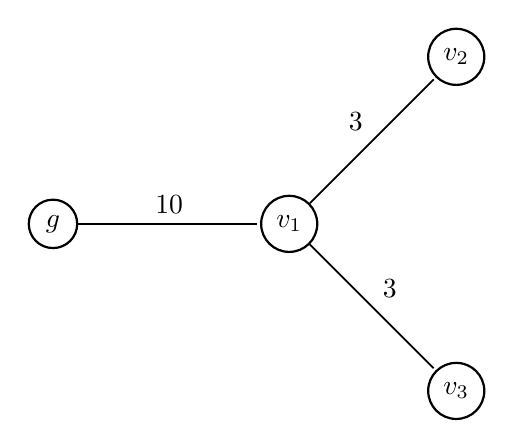
\begin{tikzpicture}[
            > = stealth,
			shorten > = 1pt,
            auto,
            node distance = 3cm,
            semithick
        ]
        \tikzstyle{every state}=[
            draw = black,
            thick,
            fill = white,
            minimum size = 4mm
        ]
        \node[state] (g) {$g$};
        \node[state] (v1) [right of=g] {$v_1$};
        \node[state] (v2) [above right of=v1] {$v_2$};
        \node[state] (v3) [below right of=v1] {$v_3$};

        \path[-] (g) edge node {10} (v1);
        \path[-] (v1) edge node {3} (v2);
        \path[-] (v1) edge node {3} (v3);
\end{tikzpicture}
\end{center}
Let $h(v_1)$ = 10, $h(v_2)$ = 1, $h(v_3)$ = 6, $h'(s)$ = true cost from s to g, and g = goal. Then, we have $h'(v_1)$ = 10, $h'(v_2)$ = $h'(v_3)$ = 13. This heuristic $h(s)$ is admissible since $h(v_1) \le h'(v_1)$, $h(v_2) \le h'(v_2)$, $h(v_3) \le h'(v_3)$. It is not consistent, however, since we have a case that invalidates the consistency property. $v_2$ is a descendant of $v_1$ so $h(v_1) \le c(v_1, v_2) + h(v_2)$. This does not hold as 10 $\nleq$ 3 + 1. 
\newpage
\section{Constraint Satisfaction Problem}
\textit{In a Constraint Satisfaction Problem (CSP) search, explain why it is a good heuristic to choose the variable that is most constrained but the value that is at least constraining.}
\\\\
It is a good heuristic to choose the most constrained variable because it is the variable with the highest probability of getting reduced to zero possibilities or backtracking. Since the most constrained variable is the one with the fewest legal values, it is important to then consider the least constraining value since it will have the highest probability of leading to success by ruling out the fewest values in the remaining variables.

\section{Minimax Procedure}
\begin{figure}[H]
\centering
\begin{minipage}{.45\linewidth}
  \includegraphics[width=\linewidth]{images/q7_1.jpg}
  \caption{}
  \label{fig:ex1}
\end{minipage}
\hspace{.05\linewidth}
\begin{minipage}{.45\linewidth}
  \includegraphics[width=\linewidth]{images/q7_2.jpg}
  \captionof{figure}{}
  \label{img2}
\end{minipage}
\end{figure}
a) Max player should choose to move to C, Min player should then choose 
their best option which is H with a final value of 4.
\\\\
minimax(root) = max(min(3,5),min(4,max(7,8),max(5,min(0,7)))) =\\ max(3,min(4,8,5)) = \\
max(3,4) = 4
\\\\
b \& c) \textbf{Figure 1} is left-to-right alpha-beta pruning while \textbf{Figure 2} is right-to-left alpha-beta pruning. Pruning occurs differently because nodes are revealed in a different order. This order may allow us to prune or ignore certain branches sooner based on how the revealed values compare in relation to the ancestors’ min or max values. In this case a right to left traversal provides a faster more optimal pruning because we can make pruning decisions earlier.
\newpage
\section{Heuristics II}
\textit{Which of the following are admissible, given admissible heuristics $h_1$,$h_2$? Which of the following are consistent, given consistent heuristics $h_1$, $h_2$? Justify your answer.}\\\\
a) $h(n) = min\{h_1(n), h_2(n)\}$ h(n) is \textbf{not admissible} because taking the minimum of two admissible heuristics has a chance of overestimating the cost of reaching the goal state. Since the minimum of two admissible heuristics is not admissible, the minimum of two consistent heuristics will \textbf{not be consistent} either.
\\\\
b) $h(n) = w*h_1(n) + (1-w)*h_2(n),$ where $0 \leq w \leq 1$. Given the definition of admissible, we have $h_1(n) \leq h'(n)$ and $h_2(n) \leq h'(n)$. For any w in the range, we'd have $h(n) = w*h_1(n) + (1-w)*h_2(n) \leq w*h'(n) + (1-w)*h'(n).$ This means the average of two admissible heuristics would be \textbf{admissible}. For consistent heuristics $h_1(n)$ and $h_2(n)$, $w*h_1(n) \leq w*[c(n,a,n') + h_1(n')]$ and $(1-w)*h_2(n) \leq (1-w)*[c(n,a,n') + h_2(n')]$. Adding these together would give $w*h_1(n) + (1-w)*h_2(n) \leq w*h_1(n') + (1-w)*h_2(n') + c(n,a,n')$ which leads to h(n) $\leq$ h(n') + c(n,a,n') so the average of two consistent heuristics would be \textbf{consistent}.
\\\\
c) $h(n) = max\{h_1(n), h_2(n)\}$. h(n) would be \textbf{admissible} since the maximum of two admissible heuristics would at least be as good of an estimate as either of them. For consistency, we can combine the definitions to get $h(n) = max\{h_1(n), h_2(n)\} \leq max\{c(n,a,n')+h_1(n'),c(n,a,n')+h_2(n')\}$ and factor out the constant to get $max\{h_1(n'),h_2(n')\} + c(n,a,n') = h(n') + c(n,a,n')$ which would satisfy the consistency property and show that the max of two consistent heuristics would also be \textbf{consistent}.
\newpage
\section{Simulated Annealing}
\textit{Simulated annealing is an extension of hill climbing, which uses randomness to avoid getting stuck in local maxima and plateaux.}
\begin{enumerate}[label=(\alph*)]
\item Hill Climbing is best suited to smooth curves, in the most trivial case the graph would be in the shape of a bell curve or normal distribution. Any graph where there is only one local optimum that also serves as the global optimum will work well for hill climbing and would make simulated annealing unnecessary.
\item When there is a jagged graph or non-smooth surface simulated annealing is not very effective. If there are very sharp jumps then randomly guessing would be expected to work as well as simulated annealing because there is nothing to anneal.
\item Based on a) and b), simulated annealing works best on smooth or semi-smooth graphs where there are multiple local optimums to navigate in search of a global optimum.
\item Rather than just returning the end state with no reference or information about the states we’ve seen; we could instead track some of the previous states and do some type of analysis of them to give a better picture of the whole process and how good or bad the simulated annealing might be. 
\item Given additional memory one approach would be to store more states per run of simulated annealing instead of storing only 2 states we could use 4 or 10 states and compare them. This should provide us with a better annealing than just additional random restarts which would be moving toward random walk.
\item You can introduce randomness into the step size to avoid taking small steps close to the end state, this would work similarly to annealing and help to avoid getting stuck in local optimums.
\end{enumerate}

\newpage
\section{Game Trees}

\begin{figure}[H]
\centering
\begin{minipage}{.45\linewidth}
  \includegraphics[width=\linewidth]{images/q10_1.jpg}
  \caption{}
  \label{fig:ex1}
\end{minipage}
\hspace{.05\linewidth}
\begin{minipage}{.45\linewidth}
  \includegraphics[width=\linewidth]{images/q10_2.jpg}
  \captionof{figure}{}
  \label{img2}
\end{minipage}
\end{figure}

We drew the game trees using \href{https://www.draw.io}{draw.io} with the following conventions: $(S_A, S_B)$ where $S_A$ and $S_B$ denote token locations, a square box for every terminal state, a circle for the game value, a question mark in a circle and a red shaded box for loop states.
\\
\textbf{Figure 1} is the game tree before the minimax algorithm has been run and \textbf{Figure 2} is the game tree afterwards as it has the backed-up minimax values in circles. Because the minimax algorithm uses DFS to evaluate the nodes, we put a question mark for the backed-up minimax value of nodes that would lead into an infinite loop.
\end{document}
